
\chapter{Logical Neural Networks}

\section{Introduction}

We will discuss an NN architecture which attempts to learn boolean functions, instead of real functions. The restricted nature of boolean functions, and their use as a mathematical description of logic, allows a intuitive way of representating causation (e.g., if for some object $x$). The models that are created to solve such a problem are known as \textit{Logical Neural Networks}\footnote{also \textit{Neural Logic Networks, Logic Tensor Networks}} (LNNs)\footnote{also NLNs, LTNs}. The subfield of ML concerned with learning solutions to logical problems with gradient-descent based methods is called \textit{Neurosymbolic Machine Learning}.

The goal of the LNNs we discuss here will be to learn the optimal assignments for boolean variables within a statement described by the language of first order logic. This parallels the goal of MLPs to learn the optimal assignments for real variables within linear layers. LNNs achieve this through continuous optimisation using the standard approach of applying SGD methods with backpropagation. 

It is interesting to note that the most widely researched approaches within the field of Artificial Intelligence (AI) until the 1990s were symbolic-based methods. There are many well studied algorithms that, given a set of logical predicates known to be true, attempt to capture the nature of the wider system in a single (ideally simple!) logical statement. These algorithms are known as Inductive Logic Programming (ILP) systems \cite{ilp}. While very useful, they were found to be computationally intractible for more complex problems, notably those in Computer Vision and Natural Language Processing. Famously, Hubert Dreyfus predicted that symbolic methods were inherently incapable of fully capturing the complexity of such problems \cite{symbolicaibad}, stating that these relied primarily on unconscious processes rather than conscious symbolic manipulations. It seems most apt, therefore, to understand the rise of Deep Learning methods in the new millenium as reliant on capturing such ``unconscious'' processes.

The aim of neurosymbolic methods are thus to be able to capture the expressiveness of Deep Learning methods, without sacrificing the interpretability afforded by understanding the model in terms of symbolic manipulations. This is a difficult task! 

\section{Real Logic}

We run into the important issue of $\{\T, \F\}$, the space of boolean values, not being continuous. One way of solving this issue is by extending the domain of possible logical assignments from $\{0,1\}$, as above, to the closed interval $[0,1]$. This is referred to as both \textit{real logic}, (as in \cite{ltn2016}, \cite{analyzefuzzy}, and much of the literature focusing on differentiable applications), and \textit{fuzzy logic} (as in most foundational literature, namely \cite{fuzzysetbook}, \cite{fuzzylogicbook}, \cite{fuzzymetabook}). Using the name ``fuzzy logic'' emphasises the importance of properties which are not relevant to the neurosymbolic architecture we will be discussing here, so we will not be using the term widely, but many of the following constructions are drawn from literature on fuzzy logic. We will discuss approaches in extending important logical operators ($\OR$, $\AND$, $\NOT$, ...) to this new boolean space, and ways we may begin to use it to learn in an interpretable way. 

To fully define a ``real logic", that is, an extension of classical logic to the space $[0,1]$, we want to define all the operators in a manner that, ideally, preserves many of the useful properties we see in the classical definition. At the very least, we want the values over the restricted domain $\{0,1\}$ to be the same as in classical logic.

It is well known that given a finite number of variables $\{x_i\mid i \in 1 , \dots, N \}$, all boolean functions (that is, functions $\phi : \{\T,\F\}^N \rightarrow \{\T,\F\}$) can be expressed in terms of the operators $\lnot$ and $\land$. Explicitly,
$$
\begin{aligned}
    a \lor b &= \lnot (\lnot a \land \lnot b) \\
    a \limply b &= \lnot (a \land \lnot b) \\
    a \lxor b &= \lnot(a \land \lnot b) \land \lnot(\lnot a \land b) \\
    a \lxnor b &= \lnot(a \land b) \land \lnot(\lnot a \land \lnot b) \\
    \forall x, \phi(x) &= \phi(x_1) \land \dots \land \phi(x_N) \\
    \exists x, \phi(x) &= \lnot(\lnot \phi(x_1) \land \dots \land \lnot \phi(x_N)) \\ 
\end{aligned}
$$

If we can extend the operators $\land$ and $\neg$ to the full domain $[0,1]$, we can therefore do so for all the above operators also. For the remainder of this section, we will specify that $\T \coloneqq 1$, and $\F \coloneqq 0$, though we will later see examples where this is not the case.

\subsection{Real Conjunction and Negation}

We will take a set of properties that apply to classical conjunction $\land$ and require that the extension $\land : [0,1]^2 \to [0,1]$ has them also. The properties are;

$$
\begin{aligned}
\text{(Associativity)}&\ (a \land b) \land c = a \land (b \land c) \\
\text{(Commutativity)}&\ a \land b = b \land a \\
\text{(Monotonicity)}&\ a \leq b, c \leq d \implies a \land c \leq b \land d \\
\text{(Identity)}&\ \forall a \in [0,1], a \land 1 = a
\end{aligned}
$$

The above are known as the \textit{T-norm axioms} \cite{tnorms}. Note that they are a strict subset of the axioms required for $([0,1], \land, \lor)$ to be a boolean algebra, namely we are missing distributivity and idempotence. In fact, it is possible to construct a real logic that preserves these properties also, but there is precisely one such logic, and as we will see, it has flaws that make it less than ideal for gradient descent. The above axioms are, however, enough for $\land$ to have the correct output for the restricted domain $\{0,1\}$. 

We can likewise define negation simply by $\lnot : x \mapsto 1 - x$. In the fuzzy logic literature, this is known as \textit{strong negation}, as there is an alternate formulation of negation that captures the intention of fuzzy logic more effectively.

It can be shown that the axioms as we have defined them allow for an infinite family of possible real logics. Some examples are given below;

\begin{center}
\begin{tabular}{ c | c c c c }
    Logic & $\land$ & $\lor$ & $\forall$ & $\exists$ \\    
    \hline
    Minimum 
    & $\min\{a,b\}$ 
    & $\max\{a,b\}$ 
    & $\min\{ x_1, \dots, x_N \}$ 
    & $\max\{ x_1, \dots, x_N \}$ \\ 
    Product 
    & $ab$
    & $1 - (1 - a)(1 - b)$
    & $\prod_ix_i$
    & $1 - \prod_{i}(1-x_i)$ \\
    Łukasiewicz
    & $\max\{a+b-1, 0\}$ 
    & $\min\{a+b, 1\}$ 
    & $\max\{\sum_ix_i - N + 1, 0\}$ 
    & $\min\{\sum_ix_i, 1\}$ \\
\end{tabular}
\end{center}
\todo{Add more logics - Drastic, Nilpotent, Schweizer–Sklar, Hamacher, Yager}

Figures \ref{fig:conjplots} shows more visually how some of these logics behave.

\begin{figure}[h]
    \centering
    \begin{subfigure}[b]{0.2\textwidth}
        \centering
        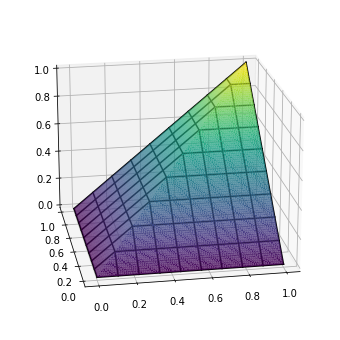
\includegraphics[width=\textwidth]{imgs/fuzzy_min_and.png}
        \caption{Minimum}
        \label{fig:minconj}
    \end{subfigure}
    \begin{subfigure}[b]{0.2\textwidth}
        \centering
        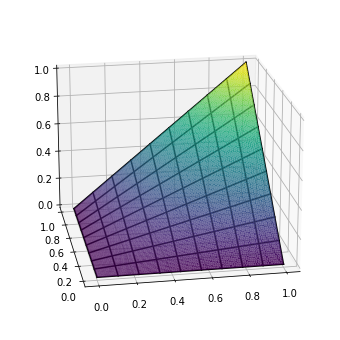
\includegraphics[width=\textwidth]{imgs/fuzzy_prod_and.png}
        \caption{Product}
        \label{fig:prodconj}
    \end{subfigure}
    \begin{subfigure}[b]{0.2\textwidth}
        \centering
        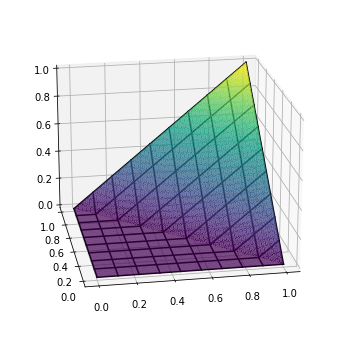
\includegraphics[width=\textwidth]{imgs/fuzzy_luk_and.png}
        \caption{Łukasiewicz}
        \label{fig:lukconj}
    \end{subfigure}
    \begin{subfigure}[b]{0.2\textwidth}
        \centering
        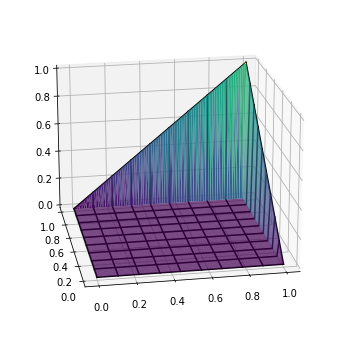
\includegraphics[width=\textwidth]{imgs/fuzzy_dra_and.png}
        \caption{Drastic}
        \label{fig:draconj}
    \end{subfigure}
       \caption{Conjunction over various fuzzy logics. Note how pointwise gradients differ.}
       \label{fig:conjplots}
\end{figure}

\section{General Architectures}

Now that we have explicit definitions for boolean-like algebras in the domain $[0,1]$, we can begin to formulate how we may learn in this setting.

We first need to consider what problems we may want to solve. A basic problem is that of \textit{satisfiability}, i.e., given a boolean function $\phi : \{0,1\}^K \rightarrow \{0,1\}$ which can be expressed in first-order logic, is there some element $\vx \in \{0,1\}^K$ such that $\phi(\vx) = 1$? If so, we want to find an example of said $\vx$.

We can consider this as a continuous optimisation problem with $\vx$ as a parameter. We can extend $\phi$ to the real domain $[0,1]$ by extending each operator in $\phi$ when expressed in the language of first-order logic. Then, by performing SGD as normal, we aim to minimise the loss function $\ell(\vx) = \lnot\phi(\vx)$.

To match the power of classical MLPs, we also want to be able to learn optimal \textit{functions} $\phi$. Suppose we have a dataset $\{(\vx_i, y_i)\}_{i=1}^N$ where $\forall i, \phi(\vx_i) = y_i$ for some formula $\phi : \{0,1\}^K  \rightarrow \{0,1\}$ which need not have a known representation in classical first-order logic. Further suppose we have a function $\psi : \{0,1\}^{K+P} \rightarrow \{0,1\}$ expressed in first-order logic such that for some $\vw \in \{0,1\}^P$, $\phi(\vx) = \psi(\vx, \vw)$. We consider $\vw$ a parameter here, and optimise for loss $\ell(\vx, y; \vw) = y \lxnor \psi(\vx, \vw)$. Extending $\psi$ to real logic as standard allows us to use continuous optimisation methods to do so. $\bbE_{\vx}[\ell(\vx, \phi(\vx); \vw)] = 0 \iff \psi(\vx, \vw) = \phi(\vx)$ for all $\vx \in \{0,1\}^K$, so the above algorithm is correct.

It is very feasible to find expressive enough $\psi$, as it can be shown that every boolean function $\phi$ can be expressed in a number of standard forms - Disjunctive Normal Form (DNF), and Conjunctive Normal Form (CNF), being two notable ones. To fit these two representations into the framework we have described, we need to be able to express how every variable $x$ is represented in each normal form by appending appropriate parameter variables $w$.

In DNF, $\phi$ is expressed as a disjunction of conjunctions, with each conjunction described by a subset of input variables $\subseteq \{x_1,\dots,x_K\}$, each variable being optionally negated. We can capture membership by boolean variables $m_i \in \{0,1\}$, and negation by $s_i \in \{0,1\}$. This allows us to represent a formula in DNF by

$$
\begin{aligned}
\phi(\vx) &= \exists j,\ 1 \leq j \leq W,\ \phi_j(\vx) \\
\text{where } \phi_j(\vx) &= \forall i,\ m_{ij} \limply (x_i \lxor s_{ij})
\end{aligned}
$$

for some assignment to the $M = (m_{ij}), S = (s_{ij})$. A similar form for CNF is,

$$
\begin{aligned}
\phi(\vx) &= \forall j,\ 1 \leq j \leq W,\ \phi_j(\vx) \\
\text{where } \phi_j(\vx) &= \exists i,\ m_{ij} \land (x_i \lxor s_{ij})
\end{aligned}
$$

In both cases, we can construct a function $\psi$ with $M$ and $S$ as parameters, and optimise over these parameters as before. Here $W \in\bbN$ is a hyperparameter which specifies the number of conjunctions (or disjunctions) in the function family $\psi$. Naturally, the larger $W$ is, the more expressive $\psi$ can be, and we know that $W = 2^K$ is enough to capture all possible functions $\phi$. This very closely parallels the Universal Approximation Theorem (UAT) of MLPs with one hidden layer.

\section{Analysis of a Toy Problem}

The framework we have given is very general, and does not specify what real logic we are required to use. Indeed it does not even require that every operation need be from the same logic, only that they are correct on classical boolean values $0,1$. It is valuable, therefore, to compare each logic and analyse which logics are useful for which learning tasks.

In \cite{analyzefuzzy}, the problem of satisfiability over $\phi(a,b,c) = (a \land b) \lor (c \land \lnot a)$ is considered. We compare the convergence of $a, b, c$ \footnote{In practice, we actually consider satisfiability over parameters $a, b, c \in \bbR$ mapped into $[0,1]$ with a sigmoid function, as we want to converge to parameters in the appropriate bounds.} over each logic, given randomly initialised starting parameters.

Figure \ref{fig:toyconv} show convergence for 1000 uniformly sampled random initialisations of the parameters $a, b, c$, using Adam optimisation \cite{adam} with a learning rate of $10^{-1}$. Convergence to $1$ represents finding a satisfying assignment, whereas anything else represents a failure to do so.

\begin{figure}[h]
    \centering
    \begin{subfigure}[b]{0.45\textwidth}
        \centering
        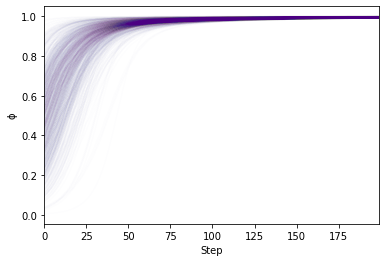
\includegraphics[width=\textwidth]{imgs/toyconv_min.png}
        \caption{Minimum}
        \label{fig:toymin}
    \end{subfigure}
    \begin{subfigure}[b]{0.45\textwidth}
        \centering
        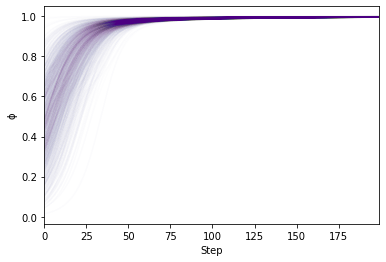
\includegraphics[width=\textwidth]{imgs/toyconv_prod.png}
        \caption{Product}
        \label{fig:toyprod}
    \end{subfigure}
    \begin{subfigure}[b]{0.45\textwidth}
        \centering
        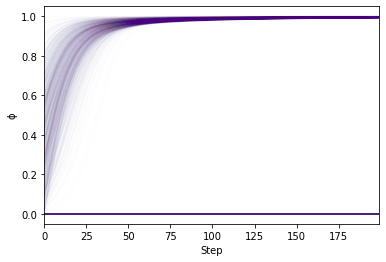
\includegraphics[width=\textwidth]{imgs/toyconv_luk.png}
        \caption{Łukasiewicz}
        \label{fig:toyluk}
    \end{subfigure}
    \begin{subfigure}[b]{0.45\textwidth}
        \centering
        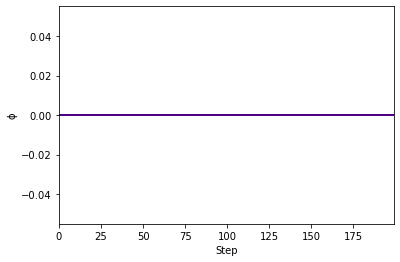
\includegraphics[width=\textwidth]{imgs/toyconv_dra.png}
        \caption{Drastic}
        \label{fig:toydra}
    \end{subfigure}
       \caption{Convergence of toy problem $\phi(a,b,c) = (a \land b) \lor (c \land \lnot a)$ for various fuzzy logics.}
       \label{fig:toyconv}
\end{figure}

We see that the choice of logic has a profound impact on the convergence. \todo{Add description of results}

\subsection{Incorrect Gradients}

It is notable that some initialisations fail to converge at all. This was also observed in \cite{analyzefuzzy}, and is very much a cause for concern. We would expect all initialisations to work, even if some converge slower than others. To investigate further, we explicitly sample observations for the gradient estimator of each parameter, to see if this can help us diagnose the issue.

\todo{Add gradient sampling tests}

\todo{Add gradient sampling analysis - ``leaky'' gradients}

By explicitly deriving the gradients for a given logic, we may begin to diagnose why this may be the case.

\todo{Derivation of gradients for product logic}

We see that this problem may be resolved by choosing a distribution of inputs that necessarily has the right sign for the expected gradient estimator. This, however, is not ideal. We would like to have a framework which provably converges in \textit{all} cases, regardless of the distribution of inputs. 

\subsection{Vanishing Gradients}

The tests further show that a majority of gradient samples are precisely $0$. It is natural that some observations would not allow us to make any meaningful inferences about the optimal values of each variable, especially in cases where the proportion of satisfying inputs is incredibly small. We observe however, that different choices of logic result in different proportions of vanishing gradient observations.

To explain this, we must discuss the nature of conjunction in each logic. The most apt example is that of Łukasiewicz logic, as for $a, b \in [0,1]$ such that $a + b - 1 < 0$, the pointwise gradient of binary conjugation $\land$ is precisely $0$. This means that a full $\frac{1}{2}$ of all possible input arguments (uniformly distributed) give no meaningful inference. Aggregating over $K$ variables, this generalises to a proportion of $1 - \frac{1}{K!}$ inputs having vanishing gradients, which is very obviously not ideal.

Therefore, in this framework, we prefer to use logics such that $\land$ has non-vanishing gradient almost everywhere. Minimum and Product logics satisfy this condition, along with certain parameterisations of the Schweizer–Sklar, Hamacher and Yager logics.

\subsection{Other Gradient Concerns}

Another consideration when comparing different logics is the phenomenon of ``partial'' vanishing gradients. The minimum logic is the best example of such - as over the entire domain, the partial derivative of conjugation is non-zero for precisely one input. This means that convergence is very \textit{binarized}, meaning only one parameter is optimised at each step. This may also have an effect on convergence, as optimisation potentially only occurs for a small subset of parameters at each step, but this may also help to remedy some of the causes of the ``leaky'' gradient problem.

\subsection{Possible Resolutions}

\todo{SGD vs Adam analysis}

\todo{Logical Dropout? In training, to regularise such that parameters are as crisp as possible, we randomly alter activations with some probability $p$ to $0$ or $1$ depending on proximity.}

\section{Comparison with Traditional Methods}

There are many well known algorithms for efficiently learning classical boolean functions $\phi : \{0,1\}^K \to \{0,1\}$ given prior knowledge of about $\phi$ restricting it to a given family. Such algorithms often make logical inferences to determine the proper state of boolean parameters $\vw$, with complexity guarantees that can be described within the Probably Approximately Correct (PAC) learning framework \cite{clt}. We will compare such algorithms to their equivalents in differentiable real logic, and hope for results as good, if not better, given an ideal optimisation regime. 

Generalising these methods to real logic would have considerable benefits. For one, given gradient descent is by nature stochastic and (aside from current parameterisation) stateless, these methods would be inherently robust to noisy data and distribution shift in the learning dataset. A possible drawback is that correctness may only be guaranteed for data drawn similarly to the training dataset, introducing a potentially unavoidable bias.

In each test, we also train a traditional MLP model on the same data. Prior to the test, we could make the assumption that the inductive bias introduced by our model could improve the rate of convergence, but an equally convincing sentiment is that this same bias could be too restrictive on the learning process, slowing down convergence.

\subsection{Learning Conjunctions}

The problem of learning conjunctions is a classical one in Computational Learning Theory (CLT). It is well known that determining conjunctions can be done PAC-efficiently \cite{clt} and is robust to noisy data \cite{noisyclt}. The goal of this comparison, therefore, is simply to prove the viability of real logic for this application.

The classical algorithm relies on one important observation. Suppose $\phi$ is a conjunction, that is - it is a function of the form 
$$\phi(x_1, \dots, x_K) = y_1 \land \dots \land y_N$$

for $y_i \in \{x_1, \dots, x_K, \lnot x_1, \dots, \lnot x_K\}$. If for some $j$, we have $\lnot x_j$ but $\phi$ returns true, then $x_j$ is not one of the terms $y_i$. Similarly $x_j \land \phi$ implies $\lnot x_j$ is not one of the terms. If we begin with $\phi$ a conjunction over all possible such terms, and remove terms where possible, we are eventually left only with the terms actually present in the conjunction.

As discussed previously, we can model the same thing in real logic by introducing weight and sign parameters $\vm$ and $\vs$, 
$$\psi(\vx; \vm, \vs) = \forall i,\ 1 \leq i \leq K,\ m_i \limply (x_i \lxor s_i)$$

and optimising $\vm$ and $\vs$.

Results using this architecture are not promising.

\begin{figure}[h]
    \centering
    \begin{subfigure}[b]{0.48\textwidth}
        \centering
        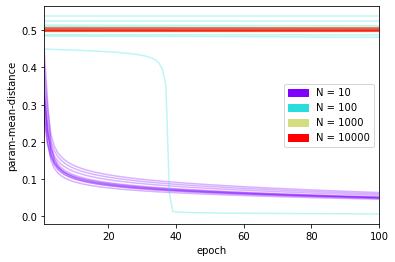
\includegraphics[width=\textwidth]{imgs/conj-pmd-prod-nokeepn-1t.png}
        \caption{1-term conjugation}
        \label{fig:conjconvnokeepn1}
    \end{subfigure}
    \begin{subfigure}[b]{0.48\textwidth}
        \centering
        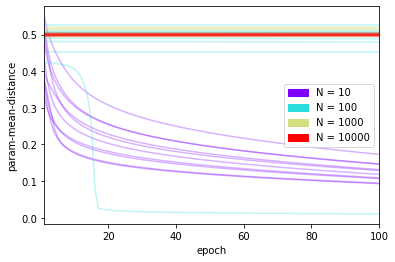
\includegraphics[width=\textwidth]{imgs/conj-pmd-prod-nokeepn-5t.png}
        \caption{5-term conjugation}
        \label{fig:conjconvnokeepn5}
    \end{subfigure}
       \caption{Convergence of mean distance from optimal parameters in learning conjugations using Product logics.}
       \label{fig:conjconvnokeepn}
\end{figure}



\todo{Add analysis, e.g. gradient stuff}

\subsection{Learning Arbitrary Functions}

An important result from CLT is that with the assumption that $\textsc{RP} \neq \textsc{NP}$, it can be shown that learning boolean functions in DNF is not PAC-efficient \textit{in general} \cite{clt}. Hopefully, relaxing boolean constraints from the discrete to the real domain allows us to overcome this issue.

\todo{Add test results here}

\todo{Add analysis}

It is important to note that 

- Suddenly not convex (much like MLP)
- Suffers greatly


\section{Alternative Frameworks}

The toy problems above show that the framework we have introduced is not adept at learning boolean functions in general. The appeal instead is that it is simple, and \textit{extensible}. A neurosymbolic layer as we have described can be embedded within a larger model, that may also contain traditional perceptron layers. These mixed models could lend their correctness to traditional NN theory, and their interpretability to their neurosymbolic aspect. In this section, we will discuss other existing neurosymbolic methods, and judge them based on the possibility of use in this application.

One common feature of many of the architectures we have not yet discussed is that logical variables $\vx$ explicitly describe some parent object. In the language of our real logic architecture, there exists some universe of objects $O$ such that boolean inputs to $\phi$ describe an object $o \in O$ in the form of a \textit{unary atom}, e.g. $\textsc{isGreen}(o), \textsc{isBig}(o)$. The output of $\phi$ can be interpreted as the valuation of a further unary predicate. Learning $\phi$ is equivalent to learning some ``if and only if" relationship between different properties of the object $o\in O$, if such a relationship exists. 

\subsection{Alternative Applications of Real Logic}

As mentioned previously, classical symbolic approaches to AI research involve the use of ILP systems. A formal description of an ILP system is one which can solve problems of the following form. Given some background knowledge $B$ of the world of objects $O$ in the form of a logical statement, and new observations of \textit{positive and negative examples} $E^+$ and $E^-$, expressed as conjugations of \textit{ground literals} (e.g. $\textsc{isGreen}(o), \lnot \textsc{areFriends}(a,b)$), we aim to find some hypothesis statement $h$ such that $B \land h$ satisfies all new observations. Formally, we require \textit{sufficiency} $B \land h \lentails E^+$, and \textit{consistency} $B \land h \land E^- \lnentails \F$ of the constructed $h$.

Our current real logic framework solves a real relaxation of the ILP problem where $E^+$ and $E^-$ are all instances of the same unary predicate. There exist differentiable real logic solvers for general ILP problems \cite{diffilp}, \cite{diffilpGT}. Such implementations improve on classical ILP methods as they are robust to noisy data while still being adept at pattern finding.

Other implementations relax real logic further by removing the requirement for all T-norm axioms to be satisfied. \cite{lnnibm} introduces \textit{Weighted Non-Linear Logic}, which is conceptually similar to Łukasiewicz logic with the addition of a bias parameter $\beta$ which is also optimised during learning. The source paper promotes this reformulation as it removes constraints from the problem of optimisation, though the algorithm introduced in the paper as stated cannot be embedded into a mixed model.

\subsection{Embedded Logic and Relations}

Many developments is neurosymbolic learning involve embedding objects into $n$-dimensional real vector spaces to exploit properties of this space. Word2vec \cite{word2vec} is a model for learning optimal embeddings of natural language atoms in a high-dimensional vector space. Such embeddings were found to preserve relationships between words through vector arithmetic \cite{word2vecrelations} (e.g. Father $-$ Man $+$ Woman $\approx$ Mother). This can be interpreted as a (relaxed) ILP system which learns over the space of \textit{binary} atoms. Learning embeddings of objects $o \in O$ in this manner will aid in extending our current real logic model to mixed models.

In \cite{ltn2016}, the notion of a \textit{grounding} is introduced - before applying any real logic operators, objects $o \in O$ are mapped into $\R^n$ through some canonical function $\calG : O \to \R^n$. An $m$-ary predicate $P$ is then interpreted as a function $\R^{n\times m} \to [0,1]$. The value of $\calG$ may then be learnt in a manner which best evaluates predicates $P$ for elements of the test dataset. 

Further, \cite{embeddedgoogle} suggests that not only should objects be embedded into a real vector space, but that boolean values should be as well. In this system, boolean values are encoded over an $n$-dimensional unit sphere $S_{n-1}$, and logical operators are required to map the encodings of $\T$ and $\F$ appropriately in this space. Introducing new dimensions may aid in improving model quality, without sacrificing interpretability as activations can be collapsed back into ``real logic'' through a similarity metric $\textsc{Sim}:S_{n-1}^2 \to [0,1]$. Cosine similarity (which corresponds to minimum distance travelling along the unit sphere) is generally used. \cite{embeddedlogicreg} improves upon this by also learning core operators $\land, \lor, \lnot$ as DNNs, with correctness ensured through regularisation rather than the architecture itself. This model has been used to develop high quality collaborative filtering algorithms \cite{embeddedcollabreasoning}.

\subsection{Bayesian Models and Probabilistic Logic}

Another approach which could be considered a continuous relaxation of classical logic is in modelling boolean values as distributions over deterministic values $\{\T, \F\}$. Bayesian methods are well studied for this application, with many efficient methods existing for learning the distributions of random variables expressed in terms of a random field. Probabilistic programming languages \cite{gordon2014probabilistic} are able to describe such problems over Bayesian Networks in an highly interpretable manner. Learning probability distributions over the parameter space $\vw$ may prove a more interpretable solution, and further may solve some of the convergence issues seen due to many problems being non-convex. If we interpret real booleans $[0,1]$ as parameters of a Bernoulli distribution over values $\{\T, \F\}$, we can analogize real logic models using the product logic to modelling a random field such that all parameters $\vw$ are independent of each other. In this interpretation, we see that using general Bayesian models increases the expressivity of our model by introducing dependencies between parameters $\vw$. Arbitrary dependencies can be modelled using Normalizing Flows \cite{normalizingflows}.

Bayesian methods are very general, and many approaches exist which are specialised for uses in logic. Bayesian networks are restrictive as they model variable dependencies as a Directed Acyclic Graph (DAG), whereas many dependencies in logic are cyclic (most notably the relation $\iff$). Markov Networks describe dependencies between random variables as edges in a graph, meaning that any two variables that are not adjacant are conditionally independent. These are used to capture logical inferences in the popular Markov Logic Network (MLN) model \cite{markovlogicnetworks}, which corresponds logical atoms to vertices, and formulae to cliques in the graph. Probabilistic Soft Logic \cite{probsoftlogic} further develops on this by introducing a PPL to describe instances of a model similar to MLNs, which can be used to better interpret the results of learning using such methods.



\begin{comment}
\section{A Useful Logical System}

\subsection{Notation}

The notation of linear algebra is very useful in succinctly describing the nature of a classical perceptron model, but within neurosymbolic layers, we do not have this luxury. Further in this paper, we will discuss many different kinds of logical systems, and we will discuss and compare their qualities in learning. To describe our models, it's useful to phrase the layers we construct in a manner similar to linear algebra.

Given a logical system $\B$, we will define a matrix/vector system much like the standard one. A boolean vector of size $n$ is an element of the set $\B^n$, and similarly a boolean matrix of height $a$ and width $b$ is an element of the set $\B^{a \times b}$. Where we now differ is in matrix algebra - in linear algebra, matrix multiplication is defined like so;
$$\mathbf{AB}_{ij} = \sum_{k}\mathbf{A}_{ik}\cdot\mathbf{B}_{kj}$$

We can define boolean matrix multiplication likewise;
$$\mathbf{AB}_{ij} = \bigvee_{k}\mathbf{A}_{ik}\land\mathbf{B}_{kj}$$

This allows us to motivate a meaning for ``dot products" also;
$$\mathbf{a\cdot b} = \mathbf{a}^\text{T}\mathbf{b} = \bigvee_i a_i \land b_i$$

It would be useful to define element-wise operations on vectors/matrices. For any operator $\circ : \B^2 \to \B$, we write $\mathbf{a} \circ \mathbf{b}$ to mean $(\mathbf{a} \circ \mathbf{b})_i = a_i \circ b_i$. If we want to apply an operator with a constant scalar value to every element of a vector, we can write this likewise, $(\mathbf{a} \circ b)_i = a_i \circ b$, etc.

Finally, if an operator $\circ$ is both associative and commutative, we write $^\circ(\mathbf{a})$ to refer to $a_1 \circ a_2 \circ \cdots$.

Using the above two, we can likewise define the ``dot product" by $\mathbf{a \cdot b} ={^\lor}(\mathbf{a \land b})$. We can use a similar notation as syntactic sugar to define matrix multiplication $\mathbf{AB} ={^\lor}(\mathbf{A \land B})$. This notation allows us to use other operators also, for example standard matrix multiplication would be written by ${^+}(\mathbf{A \times B})$. 

\subsection{Boolean Algebras}

While classical perceptron layers heavily rely on linear algebra, neurosymbolic layers cannot. Instead, we must rely on \textit{boolean algebra} to motivate our models. Boolean algebra is fundamentally different to any algebra motivated by classical arithmetic, as we do not have access to the regular operators $+$ or $\times$. Nevertheless, boolean operators behave much like arithmetic ones. A boolean algebra, formally speaking, is a mathematical object $\B$, which contains elements $\T$, $\F$, and for which we have binary operators $\lor$, $\land$, and a unary operator $\neg$, such that the following axioms always hold.

$$
\begin{aligned}
\text{(Associativity)}
&\ (a \lor b) \lor c = a \lor (b \lor c) \\
&\ (a \land b) \land c = a \land (b \land c) \\
\text{(Commutativity)}
&\ a \lor b = b \lor a \\
&\ a \land b = b \land a \\
\text{(Absorption)}
&\ a \lor (a \land b) = a \\
&\ a \land (a \lor b) = a \\
\text{(Identity)}
&\ a \lor \F = a \\
&\ a \land \T = a \\
\text{(Compliments)}
&\ a \lor \neg a = \T \\
&\ a \land \neg a = \F \\
\text{(Distributivity)}
&\ a \lor (b \land c) = (a \lor b) \land (a \lor c) \\
&\ a \land (b \lor c) = (a \land b) \lor (a \land c) \\
\end{aligned}
$$

We can immediately see the similarities to classical arithmetic. In fact, the above construct is a commutative ring, with some extra properties. 

The above system is very intuitive, as it by design can fully motivate a propositional logic. However, we have not motivated our logical system by direct construction, but by necessitating certain behaviours. We therefore need not restrict ourselves to simply the set $\B=\{0,1\}$, we can define $\B$ however we'd like, and exploit the unique characteristics of the $\B$ we have chosen in our learning.

Let's consider an alternative boolean algebra - given a set $S$, let $\B = {\{ U \subseteq S \}}$, that is, the power set of $S$. It is natural to let $\land$ be the intersection of two sets, and $\lor$ the union. We can further say $\T = S$, $\F = \varnothing$, and $\neg:U \mapsto S \setminus U$. One can immediately see that the above axioms follow from basic facts in set theory. This construction is not useful to us, however, as we cannot differentiate over it.

In practice, we'd really like not to stray too far away from classical logic $\B = \{0,1\}$, and simply approximate classical logic with our choice of $\B$. In this way, our goal is not to necessarily to exploit the properties of a boolean algebra once we have them, but to use the axioms of boolean algebras (and derivations thereof) to measure the quality of hypothetical boolean approximations we propose.

\subsection{Measuring Crispness}

To somehow measure how well our model is behaving like a boolean function, it would be useful to construct a distance metric within our space $\B$. The further away from ideal values $\T$, $\F$ we are, or from basic facts true of all boolean algebras, the worse our model may become to intuit as a logical formula.

There exist well understood ways of doing so already. A metric space $X$ is a set endowed with a \textit{distance metric} $d: X^2 \to R$ with the following properties;

$$
\begin{aligned}
\text{(Identity of Indiscernables)}
&\ d(a, b) = 0 \iff a = b \\
\text{(Symmetry)}
&\ d(a, b) = d(b, a) \\
\text{(Triangle Inequality)}
&\ d(a, b) + d(b, c) \leq d(a, c) \\
\end{aligned}
$$

For example, over classical booleans $\B = \{0,1\}$, a valid metric is $d(a,b) = a +_2 b$, where $+_2$ is addition in the finite field $\mathbb{F}_2$. This can also be interpreted as the function $\XOR(a,b) = (\neg a \land b) \lor (a \land \neg b)$. For boolean vectors $\{0,1\}^n$, a valid distance metric would be the \textit{Hamming distance} $d(\mathbf{a,b}) = {^+}(\mathbf{a} +_2 \mathbf{b})$.

For any boolean algebra $\B$, given $d$, we can define a \textit{vagueness metric}
$$v_d(a) = \min\{d(a, \T), d(a, \F)\}$$

In cases where the choice of $d$ is obvious, we will omit the subscript. We refer to values that have low vagueness as being \textit{crisp}.

\section{A General Neurosymbolic Architecture}

We will see particular implementations of LNNs later. Initially, it is important to discuss some general ideas.

As mentioned previously, the UAT shows us that it is possible to model any boolean function within the framework of MLPs, but we want to restrict the architecture of MLPs such that we could begin to interpret the learnt model as a logical formula, while maintaining full expressiveness. It is well known that any boolean function can be represented in Disjunctive Normal Form (DNF). That is, a formula that takes the form;
$$
\begin{aligned}
\phi(x_1, \dots, x_N) =\ &(a_{11} \land a_{12} \land \dots \land a_{1n_1}) \\
\lor\ &(a_{21} \land a_{22} \land \dots \land a_{2n_2}) \\ 
\lor\ &\cdots \\
\lor\ &(a_{m1} \land a_{m2} \land \dots \land a_{mn_m})
\end{aligned}
$$

where the $a_{ij} \in \{x_1, \dots, x_N, \lnot x_1, \dots, \lnot x_N\}$.

This is very convenient, as it means that any architecture we choose to build can learn this highly regular form, instead of some arbitrarily deep tree of logical operators. To transform this into the language of NNs, we want to somehow decompose the above form into a series of ``logical layers". 

There is a natural homomorphism between subsets $W \subseteq \{1, \cdots, N\}$ and disjunctions $D : \{0,1\}^n \to \{0,1\}$. That is, any disjunction $D$ is fully defined by some set $W$, where
$$D_W(\mathbf{x}) = \bigvee_{i\in W} x_i$$.

If we want to learn the disjunction $D$, it is therefore equivalent to learn the membership of the set $S$. Let $\mathbf{w} \in \B^N$, with $w_i = \mathbbm{1}(i \in S) \in \B$. Then we need only learn the value of the vector $\mathbf{w}$. It is important to note that, in the space $\B = \{0,1\}$, we have an equivalent representation

$$
\begin{aligned}
D_W(\mathbf{x}) 
&= \left(\bigvee_{i \in W} x_i\right) \lor \left(\bigvee_{i \not\in W} \F\right) \\
&= \bigvee_{i} x_i \land w_i \\
&= {^\lor}(\mathbf{w \land x}) = \mathbf{w}^T\mathbf{x}
\end{aligned}
$$

To distinguish this understanding of disjunctions with the simple operation $^\lor(\mathbf{x})$, we will refer to these as \textit{weighted disjunctions}.

This definitely justifies the notation introduced in the previous section. A similar procedure gives us a compact representation of conjunctions, though it is not as minimal;

$$
\begin{aligned}
C_W(\mathbf{x}) 
&= \bigwedge_{i \in W} x_i \\
&= \left(\bigwedge_{i \in W} x_i\right) \land \left(\bigwedge_{i \not\in W} \T \right) \\
&= \bigwedge_i \neg w_i \lor x_i \\
&= {^\land}(\mathbf{w} \Rightarrow \mathbf{x})
\end{aligned}
$$

The above notation allows us to represent boolean functions in DNF, as any formula in DNF is a disjunction of \textit{weighted conjunctions} as seen above. We write this like so.

$$F(\mathbf{x; W}) = {^\lor}({^\land}(\mathbf{W \Rightarrow x \concat \neg x}))$$

Here, $@$ is an operator representing vector concatenation.

Suppose we are given feature valuations $x_1, \dots, x_N$, and we are also given whether said features satisfy some set predicate $P(x_1, \dots, x_N)$. To create a functioning ILP system, it is enough to find some logical formula $\phi$ which is consistent with this predicate, meaning that for all inputs $\mathbf{x}$ we have received, $\phi(\mathbf{x}) = P(\mathbf{x})$. The purpose of LNNs is to use backpropagation to find an approximation to such a solution. By nature, NNs are ``forgetful" in that if the distribution and output value of incoming data changes, they are able to modify their parameterisation accordingly. They therefore aren't guaranteed to be consistent with all input data, but this actually becomes a benefit, rather than a hindrance, when we begin to embed LNN systems within classical NN architectures. 

This embedding is important to note, as the aim of the architecture presented in this paper is not to find \textit{correct} concepts, but \textit{useful} ones. We do not necessarily aim to find hypotheses that perfectly represent known concepts, but concepts that when incorporated into our decision making, allow the player of a game to perform effectively. In that sense, we are using LNNs in a way that is similar in construction, but different in intention to ILPs. This is an important distinction to make when comparing this architecture to existing ones in the space of Neurosymbolic ML, which we will discuss later.

\subsection{Interpreting a Neurosymbolic Layer}

We have constructed layers which represent learnable conjunctions and disjunctions, but how do we go about converting this into a human interpretable format? So far we have discussed an architecture which learns any boolean function in DNF, but is this an ideal way of communicating concepts to humans?

Let's consider what a formula in DNF is actually communicating. Each disjunction is naturally going to represent a single concept, and each conjunction within can be interpreted as being instances of said concept. Using the example of Chess, if we want to learn what it means for a bishop to attack a king, we want to iterate over all instances where a bishop is in a directly diagonal position to a king, with no obstruction. Determining each one of these instances can be done with a conjunction (e.g. Bishop on A1, empty spaces in B2, C3, ..., King on E5), and determining whether any of these conjunctions has occurred is handled by the disjunction. 

In this manner, the disjunction is a set of instances of a particular concept, and the conjunctions are the elements of this set.

Is this the best architecture for interpretability? One may consider an architecture with two DNF layers - that is, concepts building on top of further concepts. This can be incredibly useful - suppose we have both a bishop and a knight attacking the king. The presence of both of these concepts, one can imagine, is greater than the sum of it's parts, so it may be useful to consider this a joint concept. We don't necessarily require a second DNF layer to discover this, as we have shown that a single layer is sufficient to fully express all boolean functions, but for the sake of interpretability, it may be advantageous to add this second layer. This is in stark comparison to conventional NNs, where adding layers generally sacrifices interpretability for the sake of expressiveness. This consideration will become important when comparing different implementations of neurosymbolic architectures in practice.

We can now begin to discuss different ways of actually implementing such an architecture.

\section{Fuzzy Logic}

\def\Bf{\B_\text{f}}

An intuitive, and well researched approach to extending the space of valid boolean values is to consider truth to be ``vague", in the sense that something can be ``somewhat" true or ``somewhat" false. To quantify this, we take boolean values in the closed interval $[0,1]$, rather than simply $\{0,1\}$. This approach is known as \textit{fuzzy logic}.  From here, we will denote the traditional boolean algebra by $\B_2$, and fuzzy logic by $\Bf$. 

It is important to note that while this emulates the definition of a probability measure, it is distinctly not. $\mathbb{P}(x) = \frac{1}{2}$ states that $x$ is true with a probability of $\frac{1}{2}$, which can mean either that in $\frac{1}{2}$ of cases, $x$ appears true (the frequentist interpretation), or that we believe that $x$ is true with $\frac{1}{2}$ certainty (the Bayesian interpretation). In fuzzy logic, $x = \frac{1}{2}$ instead states that $x$ is ``half-true", with 100\% certainty. We are only using fuzzy logic to approximate classical, discrete logic, so it is not important to dwell on the philosophical implications of this. Extending the domain of boolean values means that we have to revisit the definitions of simple logical operators $\lnot, \land$ and $\lor$.

\subsection{Fuzzy Operators}

\def\prodand{\custop{\otimes_\times}}
\def\minand{\custop{\otimes_<}}
\def\lukand{\custop{\otimes_\text{L}}}
\def\draand{\custop{\otimes_\text{D}}}

\def\prodor{\custop{\oplus_\times}}
\def\minor{\custop{\oplus_<}}
\def\lukor{\custop{\oplus_\text{L}}}

We will begin with a generalisation for $\land$, as all further definitions follow from this. We want to find a function $\otimes : \Bf^2 \to \Bf$ which has the same value as $\land$ for $\B_2$, and maintains some natural properties of $\land$ also. Suppose we assume the following axioms for $\otimes$;
$$
\begin{aligned}
\text{(Associativity)}&\ (a \otimes b) \otimes c = a \otimes (b \otimes c) \\
\text{(Commutativity)}&\ a \otimes b = b \otimes a \\
\text{(Monotonicity)}&\ a \leq b, c \leq d \implies a \otimes c \leq b \otimes d \\
\text{(Identity)}&\ \forall a, a \otimes 1 = a
\end{aligned}
$$
 
The axioms are actually already enough to ensure that $\otimes |_{\B_2} = \land$. However, they are not enough to ensure $\otimes$ takes one particular value in the set $\B_\text{f}^2 \to \B_\text{f}$, in fact there are an infinite family of possible functions $\otimes$. The above axioms are known as the \textit{t-norm axioms}, and the functions which satisfy it are known as \textit{t-norms}. Some examples of t-norms are;
$$
\begin{aligned}
    \text{(Product t-norm)}&\ a \prodand b \coloneqq ab \\
    \text{(Minimum t-norm)}&\ a \minand b \coloneqq \min\{a,b\} \\
    \text{(Łukasiewicz t-norm)}&\ a \lukand b \coloneqq \max\{a+b-1,0\}
\end{aligned}
$$

If we can generalise either $\lnot$ or $\lor$, then we can generalise both. A seemingly obvious way to generalise $\lnot$ is by simply declaring that $\lnot x = (1 - x)$. This immediately satisfies the definition of $\lnot$ in classical logic, and comes with some useful properties;
$$
\begin{aligned}
\text{(Self-Invertibility)}&\ \lnot(\lnot a) = a \\
\text{(Monotonicity)}&\ a \leq b \implies \lnot a \geq \lnot b \\
\end{aligned}
$$

From this, we can fully define generalisations for $\lor$, which we call \textit{t-conorms}. In classical logic, we can appeal to \textit{De Morgan's laws}, in that $a \lor b = \lnot (\lnot a \land \lnot b)$. Similarly, we can say that $a \oplus b = \lnot(\lnot a \otimes \lnot b) = 1 - (1 - a) \otimes (1 - b)$, given a particular choice of t-norm $\otimes$. We therefore have;

$$
\begin{aligned}
    \text{(Product t-conorm)}\ a \prodor b \coloneqq &\ 1 - (1-a)(1-b) \\
    = &\ a + b - ab \\
    \text{(Minimum t-conorm)}\ a \minor b \coloneqq &\ 1 - \min\{1-a,1-b\} \\
    = &\ \max\{a, b\} \\
    \text{(Łukasiewicz t-conorm)}\ a \lukor b \coloneqq &\ 1 - \max\{(1-a)+(1-b)-1,0\} \\
    = &\ \min\{a+b, 1\}
\end{aligned}
$$

Given the t-norm axioms, we immediately have some convenient properties of t-conorms also.

$$
\begin{aligned}
\text{(Associativity)}&\ (a \oplus b) \oplus c = a \oplus (b \oplus c) \\
\text{(Commutativity)}&\ a \oplus b = b \oplus a \\
\text{(Monotonicity)}&\ a \leq b, c \leq d \implies a \oplus c \leq b \oplus d \\
\text{(Identity)}&\ \forall a, a \oplus 0 = a
\end{aligned}
$$

The only difference here being that the identity has value 0, rather than 1. From this, we can define every logical formula using fuzzy logic operators, allowing us to motivate an architecture for a fuzzy NN.

In the field of fuzzy logic, the above method of constructing fuzzy operators is not actually the preferred way of doing so. Fuzzy logicians instead choose to define the \textit{residuum} $\Rightarrow$ in terms of fuzzy conjunction $\otimes$. The residuum, as the symbol suggests, is meant to generalise the implication operator $(a \Rightarrow b) = \lnot(a \land \lnot b)$. The reason this can be done only relying on the existence of the t-norm (rather than t-norm + fuzzy negation) is because it can be proven that the residuum is the \textit{only} function that satisfies the conditions
$$a \otimes b \leq c \iff a \leq (b \Rightarrow c)$$

The justification for this fact comes from the understanding of fuzzy logic as measuring ``confidence" - if we have confidence valuations for $a, a \Rightarrow b \in \B_f$, and we know that $a, a \Rightarrow b$ entails $b$ in classical logic, then we would expect to be at least $a \otimes (a \Rightarrow b)$ confident in $b$, i.e. that $a \otimes (a \Rightarrow b) \leq b$. A similar construction results in the conclusion above, and allows us to uniquely determine $\Rightarrow$. From here, we can choose to define the other logical operators like so;

$$
\begin{aligned}
\lnot a =&\ (a \Rightarrow 0) \\
a \oplus b =&\ (\lnot a \Rightarrow b)
\end{aligned}
$$

Again, we will not dwell on this, as we are aiming to construct fuzzy operators specifically to approximate classical logical formulae in DNF. The definitions for negation, conjunction and disjunction given above are more than enough to begin doing so. In the notation introduced previously, we could write a formula for a fuzzy DNF layer like so.
$$
F(\mathbf{x, W}) = {^\oplus}({^\otimes}(\mathbf{W \Rightarrow x \concat \neg x}))$$

\subsection{Constructing Fuzzy Operators}

So far we have declared the existance of operators satisfying the given axioms, but we have not discussed how we might discover new ones. It is important to be able to do so freely, as the convergence rate of an algorithm may have a strong relation to the gradient of the chosen operator. To give an example, an operator known as the \textit{drastic t-norm} is 0 anywhere it doesn't have to be anything else, i.e.
$$a \draand b = \begin{cases}
    a &\text{if } b = 1 \\
    b &\text{if } a = 1 \\
    0 &\text{otherwise}
\end{cases}$$

The gradient of $\draand$ is 0 almost everywhere, which isn't terribly ideal for gradient descent. We want to be able to avoid cases like this, and to do so it would beneficial to come up with a method to construct t-norms reliably. Suppose we had a decreasing function $f:\Bf \to [0,\infty]$ with $f(1)=0$. Then the function $T(a,b) = f^{-1}(\min\{f(0), f(a) + f(b)\})$ is a t-norm - in fact, most common t-norms can be constructed in this way. This statement omits some details, but for our use cases this is fine.

A function $f$ which begets a t-norm in this manner is called an \textit{additive generator} of the t-norm. Some examples are;

$$
\begin{aligned}
\text{(Product t-norm)} &\ f(x) = -\log(x) \\
\text{(Łukasiewicz t-norm)} &\ f(x) = 1 - x \\
\text{(Drastic t-norm)} &\ f(x) = 2 - x \text{ for } x \in [0,1), f(1) = 0\\
\end{aligned}
$$

This characterisation of t-norms also allows us to explicitly define conjunctions over many variables - if $a \otimes b = f^{-1}(\min\{f(0), f(a) + f(b)\})$, then ${^\otimes}(\mathbf{x}) = f^{-1}(\min\{f(0),{^+}(f(\mathbf{x}))\})$. Thus,

$$
\begin{aligned}
^\prodand(\mathbf{x}) &= {^\times}(\mathbf{x}) \\
^\lukand(\mathbf{x}) &= \max\{0, 1 + {^+}(\mathbf{x} - 1)\}
\end{aligned}
$$


and so on. In the construction of t-norms from additive generators, we have to add a $\min$ operation, as the sum $f(a) + f(b)$ may be out of the range of $f$. If there exist $a,b \neq 0$ such that this is the case, we refer to the corresponding t-norm as \textit{nilpotent}, since $a \otimes b = 0$. More accurately, this name arises due to the fact that for such $a \neq 0$, there exists $n \in \N$ such that $\underbrace{a \otimes \cdots \otimes a}_{n \text{ times}} = 0$. 

Examples of nilpotent t-norms are the Łukasiewicz t-norm $\lukand$, and the drastic t-norm $\draand$. In fact, any t-norm whose additive generator is continuous around $0$, and doesnt cover the full possible range $[0, \infty]$, is nilpotent in this manner. Any nilpotent t-norm has a non-negligible region of zero gradient, so this will help inform our future discussion on constructed t-norms.

\subsection{Defuzzification and Interpretation}

Suppose we have embedded a fuzzy LNN layer into our larger neural network. How do we go about interpreting the parameterisation of the function? We have already discussed how we may approach doing so for classical DNFs, but to achieve anything at all, we would need to be able to do so for fuzzy DNFs as well.

We can avoid this issue by ensuring that we learn parameters that are as close to $\B_2$ as possible. To do so, we may consider applying some regularisation term to our loss function, which negatively weights parameter values that are not very crisp. We could then add a regularisation term $\lambda \sum_w v(w)$ over all parameters $w$, and use cross-validation to find an optimal $\lambda$ for learning.

In practice, this hinders learning quite a bit. Much of the strength of fuzzy logic architectures are a direct result of maintaining vagueness - if we are close to values $0$, $1$, it can take a lot of data to modify this.

A more effective approach in practice seems much more naive - that is to simply clamp the value of the parameters $w$ into the range $[0,1]$ at every optimisation step. This allows the model to maintain a level of vagueness where it cannot learn much information, i.e. not ``jumping to conclusions". When it actually can decide the nature of a concept, it can freely do so. We may then choose to terminate our learning when the parameters are sufficiently close to values $\{0,1\}$.

In future sections, we see that using the distance metric $d$ \textit{can} be quite effective in regularisation, but not for directly ensuring crispness - we will use the function $v$ to evaluate the interpretability of our chosen models, but we will not actively optimise for interpretability, we want the models to passively approach crisp parameterisations.

\section{Parameterised Logic}

So far, we have discussed learning the membership of conjunctions and disjunctions only, while keeping the actual definitions of operators constant. We have discussed the fact that some choices of operators may be more successful in learning through backpropagation than others, with the case of the drastic t-norm $\draand$ being a particularly bad choice. How may we find the \textit{most successful} one? 

It's difficult to quantify what this means, so we will not attempt to do so. Instead, we can find some way of defining parameterised \textit{families} of logical systems, and learn the optimals parameters of these families in the same way we learn the parameters of the formulae we are trying to learn.

\subsection{Parameterised T-Norms}

In the previous section, we discussed an easy way to construct new t-norms, so it would make sense to use this technique here. We would like to find a family of t-norms that are all parameterisations of a more general construction. We can begin by parameterising additive generators, and constructing their respective t-norms likewise.

Let $f_p(x) = \frac{1 - x^p}{p}$. This satisfies all the criteria for an additive generator, since $f_p'(x) = -x^{p-1} \leq 0$, and $f_p(1) = 0$. For $p=0$, this is not well defined, but taking the limit as $p$ approaches 0 allows us to extend the function further. In fact this limit is well known - we can say that $f_0(x)=-\log x$, which is actually the additive generator for the product t-norm $\prodand$. What is the resultant t-norm in general?

Since $f^{-1}_p(x) = (1-px)^\frac{1}{p}$, we have $a \otimes_p b = \max\{0, (x^p + y^p - 1)^\frac{1}{p}\}$, and more generally, ${^{\otimes_p}}(\mathbf{x}) = \max\{0, (1 - {^+}((1 - \mathbf{x})^p))^\frac{1}{p}\}$. Of note is that, for $p=1$, this is the Łukasiewicz t-norm $\lukand$. It seems as though many t-norms we have already encountered are members of this family. Indeed, if we further extend the definition we have to $-\infty, \infty$ via continuity, we discover that $\otimes_{-\infty}$ is the minimum t-norm, and $\otimes_\infty$ is the drastic t-norm.

This is wonderful news, as it means with one parametric family of t-norms, we can capture all the examples we might like to study, and then some. These operators are known as the \textit{Schweizer–Sklar t-norms}. Some more parameterised families of t-norms are given by the following additive generators;

$$
\begin{aligned}
\text{(Yager t-norms)}&\ f(x) = (1-x)^p \\
\text{(Aczél–Alsina t-norms)}&\ f(x) = (- \log x)^p \\
\text{(Hamacher t-norms)}&\ f(x) = \log\frac{p+(1-p)x}{x}
\end{aligned}
$$

\subsection{Biased Logic}

There are many properties of classical logical operators that cannot necessarily be captured by fuzzy operators. \textit{Idempotence} is a resultant property of both $\land$ and $\lor$ in boolean algebras, which specifies that for all $a, b \in \B_2$, $(a \land b) \land b = (a \land b)$, and likewise for $\lor$. For most t-norms, this is specifically not the case - an obvious example is the product t-norm, where $abb=ab \iff b = 1$. It would be nice to preserve idempotence, but this is not really required. What if we can sacrifice other properties of boolean operators as well?

We will introduce a new parameterised family of boolean operators, called \textit{weighted non-linear logic} (WNL). WNL is a generalisation of Łukasiewicz logic which introduces a bias term $\beta$, which mirrors the bias used in perceptron layers of classical NN architectures. 

We will define conjunctions and disjunctions like so 



\subsection{Boolean Regularisation}

\subsection{Measuring Similarity}

\section{General Boolean Embeddings}

So far we have met Fuzzy Logic, which fundamentally reinvents the common perceptron architecture seen in most NNs. What if we want to maintain an architecture which is more conventional in it's approach, while still allowing for boolean interpretations? This seems difficult at first - although we can approximate any boolean function, determining the nature of this function is difficult in conventional architectures, as we have seen.

Rather than modifying the architecture of the network, we can instead regularise an existing network architecture to act like a boolean function, while making sure that the regularisation somehow allows us to easily interpret the network's parameters. This sounds rather involved - how might we begin to approach this?

\subsection{Booleans as Vectors}

We have discussed the idea of embedding values representing $\T$ and $\F$ into a continuous space $\B$, and then differentiating over the space in backpropagation. In fuzzy logic, we specifically fix the set $\B_\text{f}\coloneqq[0,1]$ to act as our continuous space, and exploit this by using continuous functions which are guaranteed to behave like logical operators. What if we instead allow for the full range of parameters $\R$, how may we begin to interpret this as a boolean function?

We can take inspiration from other architectures where feature embeddings are common. In natural language processing, word embeddings are maps which take words in a dictionary, and map them into a finite-dimensional vector space. The position the word is mapped to in this vector space can be used to characterise the meaning of the word, and capture relations between words. We could likewise map the boolean values $\T$, $\F$ into a vector space $\B$, and measure the ``crispness" of a learnt function by how similar certain values are to the boolean embeddings in this vector space.

We can define some sort of ``distance metric" over $\B$, a convex, commutative function $d : \B^2 \to \R$ such that $d(\mathbf{a, a}) = 0$ for all $\mathbf{a} \in \B$. This can be a formal distance metric in the topological sense, but it need not be. With this, we can say that the more distant a value $\mathbf{x} \in \B$ is from both $\T$ and $\F$, the less crisp. A particular example which is effective in practice is given later in this section.

\subsection{Learning a Boolean Operator}

Suppose we want to learn the function $\XOR(a, b) = (a \land \lnot b) \lor (\lnot a \land b)$. The model we will use to approximate this will be a NN with a single hidden layer, as it is well known that this cannot be done by a simple single-layer perceptron model. The model will therefore map values between three spaces, which we will call $\B^2 \to X \to \B$, for some $\B, X$, which we will not yet specify.

From here, we can proceed as usual and simply backpropagate with correct input-output pairs to learn an appropriate parameterisation for $\XOR$. However, we can somewhat cheat, because we know the appropriate behaviours of the function we're trying to learn, we only want to learn it over our arbitrary boolean embedding $\B$. We can exploit known properties of $\XOR$ to ``push along" our learning. For instance, we know that;

$$
\begin{aligned}
\text{(Associativity)}&\ \XOR(\XOR(\mathbf{a, b}), \mathbf{c}) = \XOR(\mathbf{a}, \XOR(\mathbf{b, c})) \\
\text{(Commutativity)}&\ \XOR(\mathbf{a, b}) = \XOR(\mathbf{b, a}) \\
\text{(Identity)}&\ \forall \mathbf{a} \in \B, \XOR(\mathbf{a}, \F) = \mathbf{a} \\
\text{(Negation)}&\ \forall \mathbf{a} \in \B, \XOR(\mathbf{a}, \T) = \lnot \mathbf{a}
\end{aligned}
$$

The meaning of $\lnot\mathbf{a}$ here will be explained the next section. We will define a ``$\XOR$-iness loss",
$$\ell_\XOR(\mathbf{x,y}) = d(\XOR(\mathbf{x, y}),\XOR(\mathbf{y, x})) + d(\XOR(\mathbf{x}, \F), \mathbf{x}) + d(\XOR(\mathbf{x}, \T), \lnot \mathbf{x})$$

We can see that a perfect parameterisation of $\XOR$ would minimise this loss. Thus, a complete loss function would look like so,
$$\ell(\mathbf{x,y,z}) = d(\XOR(\mathbf{x,y}),\mathbf{z}) + \lambda_\XOR \ell_\XOR(\mathbf{x,y})$$

The parameters of $\XOR$ are hidden in this representation, as they need not be of any particular architecture.

\subsection{Measuring Similarity}
 
\section{Overview of Different Architectures}
\end{comment}